\documentclass[12pt,a4paper]{article}
\usepackage[utf8]{inputenc}
\usepackage[english, russian]{babel}

\usepackage{comment}

\usepackage{amsmath}
\usepackage{amsfonts}
\usepackage{amssymb}
\usepackage{url}
\usepackage[left=1cm,right=1cm,top=1cm,bottom=1cm]{geometry}
\usepackage{graphicx}

\DeclareMathOperator{\Var}{Var}
\DeclareMathOperator{\E}{E}


\begin{document}
\thispagestyle{empty}

Here $W_t$ always denotes the standard Wiener process. 

\vspace{10pt}

\begin{enumerate}


\item $[$10 points] Let $\tau$ denote the first moment of time when $|W_t|=100$. 
\begin{enumerate}
\item What is the distribution of $W_{\tau}$?
\item Are $W_{\tau}$ and $\tau$ independent?
\item Assuming that some version of Doob's theorem may be applied find $\E(e^{-2\tau})$. 
\end{enumerate}
Hint: maybe $\exp(2 W_t - 2 t )$ will help?


\item $[$10 points] The random variables $X_1$, $X_2$, \ldots, $X_n$, \ldots are independent uniformly distributed on $[0; 1]$. I am summing them until the first $X_i$ greater than 0.5 is added. After this term I stop. Let’s denote by $S$ the total sum and by $N$ --- the number of terms added. Find $\E(S|N)$, $\Var(S|N)$, $E(S)$ % , $Var(S)$.

Hints: If $U$ is uniform on $[a;b]$ then $\Var(U)=(b-a)^2/12$. If $G$ has geometric distribution (the number of throws to get the first success) then $\E(G)=1/p$  where $p$  is the probability of success.

\item $[$10 points] Find $\Var\left(  \int_0^t W_s \, ds  \right)$. 

You may use the following guiding steps:

\begin{enumerate}
\item Find $d(tW_t)$ in short and full forms
\item Find $\E\left(2t W_t\int_0^t s \, dW_s\right)$
\item Find $\E\left(\left(\int_0^t s \, dW_s\right)^2 \right)$
\item Find $\E\left(  \int_0^t W_s \, ds  \right)$
\item $(a-b)^2=a^2-2ab+b^2$ :)
\end{enumerate}

\item $[$10 points] The risk-free interest rate is equal to $0.1$. The volatility of the share is equal to $\sigma=1$. You have an option to receive 1\$ two years later if the percentage change of price during the first year is less than during the second year. Assume the framework of the Black and Scholes model. What is the fair price of this option?

\item $[$20 points] Solve the stochastic differential equation 
\[
dX_t = t \, dt + X_t \, dW_t, \; X_0=1
\]

You may use the following guiding steps:
\begin{enumerate}
\item Solve a less difficult stochastic differential equation, $dY_t=-Y_t \, dW_t, \; Y_0=1$
\item Find $dA_t$, where $A_t=X_t Y_t$ 
\item Find any deterministic function $f(t)$ such that $d(f(t) A_t)$ contains neither $X_t$ nor $A_t$
\item Using full form of $d(f(t) A_t)$ find $X_t$. It may depend on some integrals :)
\end{enumerate}

\end{enumerate}

\begin{center}
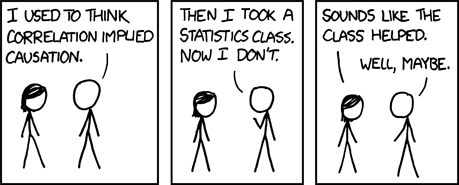
\includegraphics[width=12cm]{correlation.png} 
\end{center}



\begin{comment}
\begin{enumerate}
\item $W_{\tau}$ takes values $100$ and $-100$ with equal probabilities. Yes, independent. $\E\left(  e^{-2\tau} \right) = \frac{2}{e^{200}+e^{-200}}$
\item $\E(S|N)=0.25N+0.5$, $\Var(S|N)=0.25N/12$, $\E(N)=1/p=2$, $\E(S)=\E(\E(S|N))=1$, $\Var(S)=1/8+1/24=1/6$
\item By hints:
\begin{enumerate}
\item $d(tW_t)=t \, dW_t+W_t \, dt$
\item $\E\left(2t W_t\int_0^t s \, dW_s\right)=t^3$ using Ito's isometry
\item $\E\left(\left(\int_0^t s \, dW_s\right)^2 \right)=t^3/3$ using Ito's isometry
\item $\E\left(  \int_0^t W_s \, ds  \right)$
\item $\Var\left(  \int_0^t W_s \, ds  \right)=t^3/3$
\end{enumerate}
\item Event $\left\{ \frac{S_1-S_0}{S_0} < \frac{S_2-S_1}{S_1} \right\}$ simplifies to $S_1^2<S_0 S_2$ and further simplifies to $2\tilde{W}_1 - \tilde{W}_2 < 0$.

And 
\[
X_0=e^{-0.2}\tilde{P}(2\tilde{W}_1 - \tilde{W}_2 < 0) = e^{-0.2}/2
\]

\item By steps:

\begin{enumerate}
\item $Y_t=\exp(-W_t-t/2)$
\item $dA_t= Y_t (t-X_t)dt$
\item $f(t)=e^t$ for example
\item 
\[
X_t=\frac{1+\int_0^t s \exp(-W_s+s/2) \, ds}{ \exp(-W_t +t/2 )}
\]
\end{enumerate}


\end{enumerate}
\end{comment}



\end{document}